\chapter{Contribution}
\label{sec:contribution}

In the following chapter, contribution during Master Thesis is presented.
As result, a GNN can be presented which is called \textit{GAT-Denoiser}.
It main components and the overall architectur, will be explained in the current chapter.

The focus during practical part was on classical computed tomography in 2D but
can be generalized to cryo-EM and 3D.


\paragraph{Goal}
As introduced in chapter~\ref{sec:imaging}, molecular imaging methods computed tomography and cryo-EM are the problems
to approach. Further, the high-noise regime is the domain of interest, to be more precise SNR between $[-20, 0]$.

For a given set of observations (many sinograms or micrographs), a GNN will be trained, such that
it enables denoising of observations which are expected to have better reconstruction results.
The trained model allows to denoise not seen observations, which are from the same family of observations.


\begin{tcolorbox}[colback=red!5!white,colframe=red!75!black]
  To start solving the problem, an algorithm was designed to work with computed tomography, further
  projection angles are assumed to be known and $\theta$ was defined as equally spaced points on the unit-circle. \\

  Therfore, in the following chapters the main focus will be on computed tomography. 
  But, the concept of the algorithm would work in 3D, so for cryo-EM as well.
\end{tcolorbox}

\paragraph{Input graph:}
To recap from section~\ref{sec:graphConstruction}, our graph from molecular-imaging observation
will have single observations as nodes (one horizontal line of the sinogram). 
As $\theta$ is fixed, angle corresponding to each single observation are known. 
Based on these angles, neighbouring nodes can be connected.



\section{Components}
In the following section, the components of GAT-Denoiser are introduced. 
GAT-Denoiser is a graph neural network and the main component is a GAT. 
The main idea of GAT-Denoiser is to enable denoising of observations:
\begin{equation}
  \text{GAT-Denoiser} (\cdot) : L^2(\tilde{\Omega}) \to  L^2(\tilde{\Omega}) , y \mapsto \text{GAT-Denoiser} (y) 
\end{equation}

The GAT is expected to denoise observation signal with its neighbours by averaging. 
Further, convolution is added to denoise single observations.


But, the main overall goal is to get the best possible reconstruction 
from noisy observation $y$ which approximates original object $x$ and 
not just denoise observation $y$ which approximates noiseless observation $p$.


\begin{equation}
  x \approx   Recon \left( \text{GAT-Denoiser} \left( y \right) \right)
\end{equation}

Therefore, an end-to-end learning approach is used where quality of reconstruction is 
compared in the loss during GAT-Denoiser training, which is expected to perform better than 
only optimizing denoising of observations.

\paragraph{Fixed projection angles}
As already mentioned, projection angles are assumend to be fixed and equally spaced on the unit-circle.
This assumption is pretty strong, but good to start with developing an algorithm.

\begin{tcolorbox}[colback=red!5!white,colframe=red!75!black]
  For our GNN, this means that graph topology is fixed. 
  A K-NN graph can be built from points, equally spaced on the unit-circle,
  as signal of observations is assumed to process the low-dimensional manifold.
\end{tcolorbox}



\subsection{Graph Attention Networks}
The main component of our GNN is a GAT.
As mentioned in section~\ref{sec:graph_depp_learning}, GAT is an extension to GCN and 
adds attention (or weights) to neighbours for learning new node feature representations. 
Again, topology of the graph will no change but weighted averaging over the neighbourhood 
will take place and this is what in denoising is a good idea.

\paragraph{Single Layer}
Input of a single GAT layer are node features $h = \{ h_1, h_2, \dots , h_N \} \in \mathbb{R}^F$, 
where $N$ is the number of nodes and $F$ the number of features per node. 
The layer will map input to output, which can potentially have different dimensions: 
$h^{\prime} = \{ h_1^{\prime}, h_2^{\prime}, \dots, h_N^{\prime} \} \in \mathbb{R}^{F^{\prime}} $

As is other GNNs, input features are initially 
linearly transformed and parametrized by a learnable weight matrix $W \in \mathbb{R}^{F^{\prime} \times F}$.
This allows to add enough expressiveness to the neural network and weights are learned during training.

Further, attention coefficiants are computed, which indicate the importance of node $j$ to node $i$:

\begin{equation}
  e_{ij} = a(Wh_i, Wh_j),
\end{equation}

with $a$ as the shared attentional meachanism $a : \mathbb{R}^{F^{\prime}} \times \mathbb{R}^{F^{\prime}} \mapsto \mathbb{R}$.
But how to define the attentional mechanism? 
\citet{GAT} proposed to use a single-layer feedforward neural network, paremetrized by a weight vector $a \in \mathbb{R}^{2F^{\prime}}$
and LeakyReLu as activation function, which is good to start with.
 
Coefficients $e$ need to be normalized, such that all attention coefficient of one node sum up to 1 and therefore are comparable nicely across nodes.
Therefore, softmax is used as normalization and normalized attention coefficient are defined as:
\begin{equation}
  \alpha_{ij} = softmax_j(e_{ij})
\end{equation}


Finally, the new node embedding is calculated as:

\begin{equation}
  h_i^{\prime} = \sigma \left( \sum_{j \in \mathcal{N}_i} \alpha_{ij} W h_j \right),
\end{equation}

with $\sigma$ as some arbitrary activation function.

\paragraph{Multi-Head attention}
Motivated by \citet{transformer}, multi-head attention can be beneficial to stabilize learning process.
Therefore, not only single weight matrix is learned but it is splitted up in several parts, 
all learned individually:

\begin{equation}
  h_i^{\prime} = \bigparallel^K_{k=1} \sigma \left(\sum_{j \in \mathcal{N}_i} \alpha_{ij}^k W^k h_j \right),  
\end{equation}

where $\parallel$ corresponds to concatenation, $\alpha_{ij}^k$ the $k$-th attention mechanism and $W^k$ the linear
transformations weight matrix. The final output consists of $KF^{\prime}$ output features.

\paragraph{Last layer:}
If working with multiple heads, in the last layer of our neural network, concatenation is not the desired 
way to prepare output and therefore, averaging instead of concatenation is used.

\subsection{Convolution}
The second key component of our GAT-Denoiser is convolution.
Convolution is an important part in Signal Processing, if not the most important one.
It allows to average an incoming signal, further, it is very popular in computer vision.
It commonly operators on pixel spaces, where every observation location or time slot gets one value assinged.

\begin{equation}
  x \star k = y,
\end{equation}

where $x$ is input signal, $k$ is kernel, $\star$ the convolution operator and $y$ the convolved signal.

To do convolution, a kernel size and its weights needs to be defined. 
This kernel will then slide over the input signal $x$ and computes the dot product with its weights.

In figure~\ref{fig:1d-convolution} an illustration of 1D convolution can be seen. In this example,
kernel size is set to 3 and input singal dimension $n = m + 2$. The concept of convolution can be
extended to arbitrary dimensions.

\begin{figure}[H]
  \centering
  \label{fig:1d-convolution}
  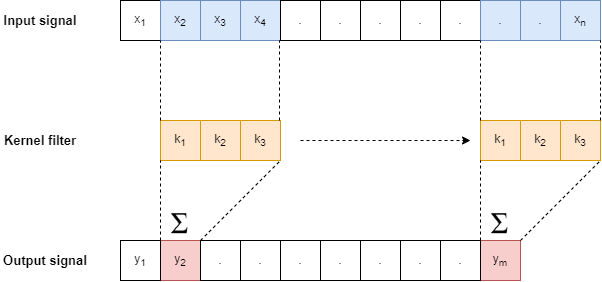
\includegraphics[width=0.4\textwidth]{Convolution.drawio.png}
  \caption{1D Convolution}
\end{figure}

\paragraph{Padding:} 
can be defined to add pixels to the boundary of the singal.
In the example, padding is set to $0$ and therefore, the signal dimension is decrased by 2.
If signal dimension should keep its dimension, padding is a powerful tool. Here, padding $1$
would keep input dimension $n$ equal to output dimension $m$.


\paragraph{Stride:}
is the parameter, how far the kernel moves each time. In our example, stride was defined to be $1$.
If stride is increased, the output signal dimension will decrease.


\subsection{U-Net}
U-Net can boost the performance of computed tomography reconstruction, compared to only using FBP.
It is an convolutional neural network, which is well suited for image segmentation in different domains.
\cite{unet-tomography} showed great success for biomedial image segmentation.

The neural network architecture consists of the contracting path and the expansive path,
resulting in a U-shape, and therefore the naming \cite{unet-tomography}, as illustrated in figure~\ref{fig:u-net-architectue}.

\begin{figure}[H]
  \centering
  \label{fig:u-net-architectue}
  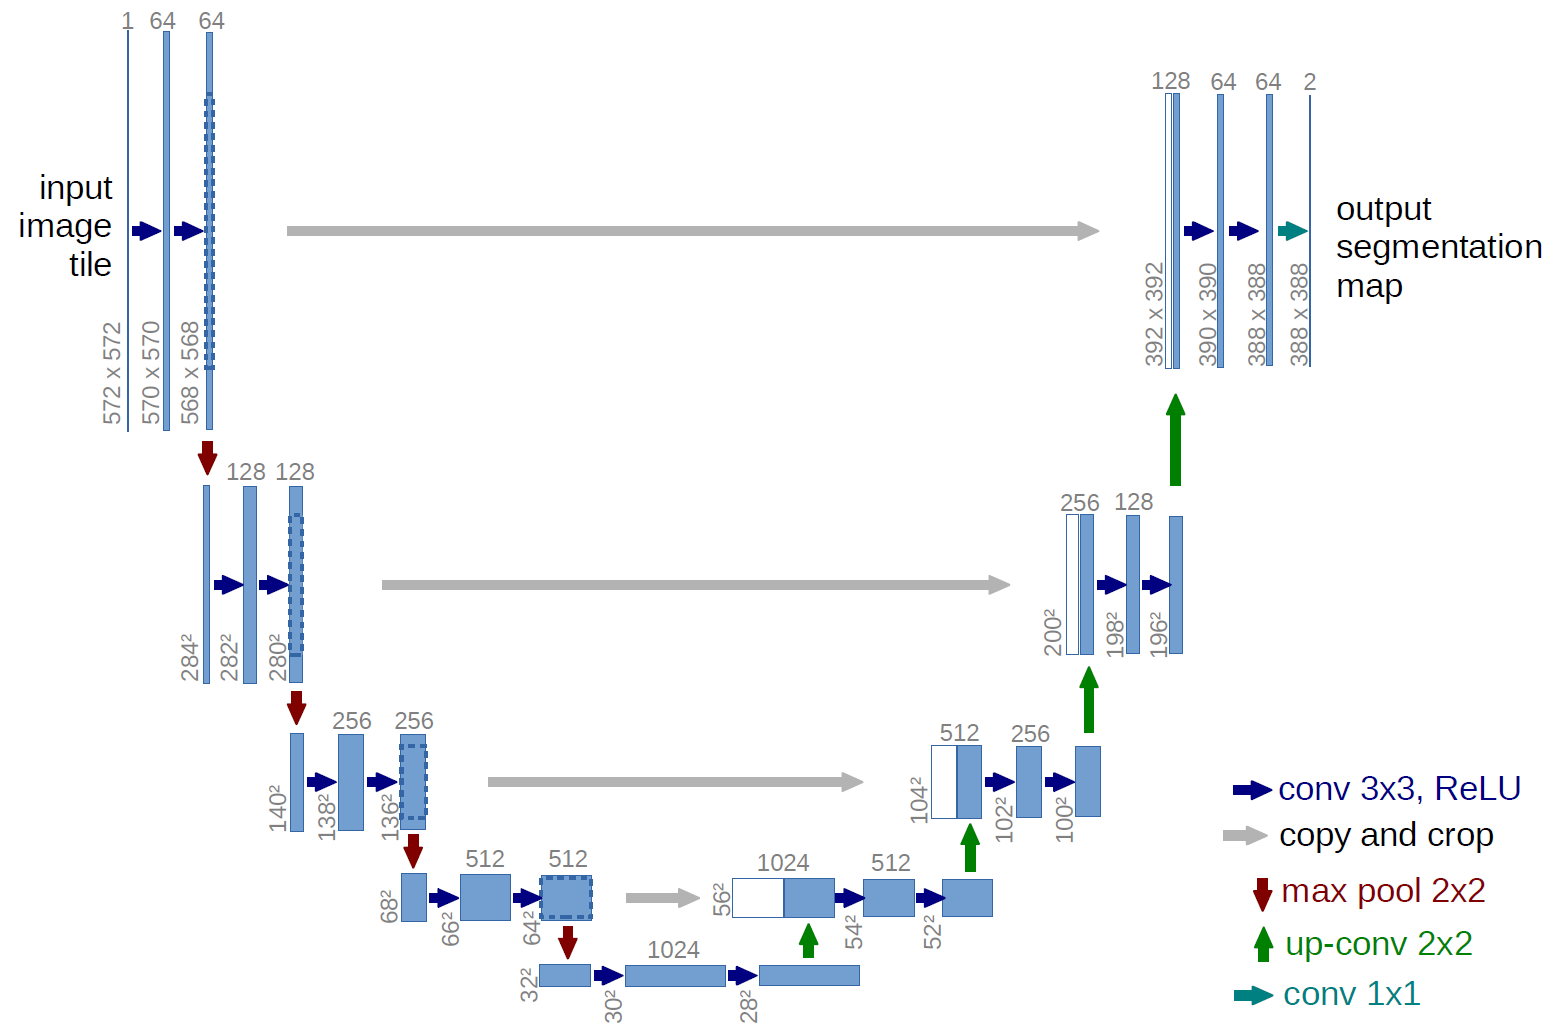
\includegraphics[width=0.6\textwidth]{u-net-architecture.png}
  \caption{U-Net architecture \cite[p 2, Fig. 1]{unet-tomography}}
\end{figure}


In the contracting path (left part), input dimension will be decreased and channels increased.
For every step in the contracting path, two 3x3 convolution layers are followed by a rectified linear unit (ReLu)
and a 2x2 max pooling for downsampling. Further, at each downsampling step, input channels are doubled.
Multiple contracting steps are combined. After last contracting step, expansive path (right part) starts
where input dimension will be increased and input channels will be decreased.
For every expansive step, an upsampling of the feature map takes place, followed by a 2x2 convolution
for up-sampling, which halves the number of channels. Then, concatenation with the corresponding feature
map of contracting path is done (gray arrow in figure~\ref{fig:u-net-architectue}), followed by again two 3x3 convolutions, followed by ReLu.
Final layer is a 1x1 convolution, to map to desired output dimension.

\section{Architecture}
Now, all individual components are introduced, the overall architecture can be defined.


\begin{figure}[H]
  \centering
  \label{fig:architecture-overall}
  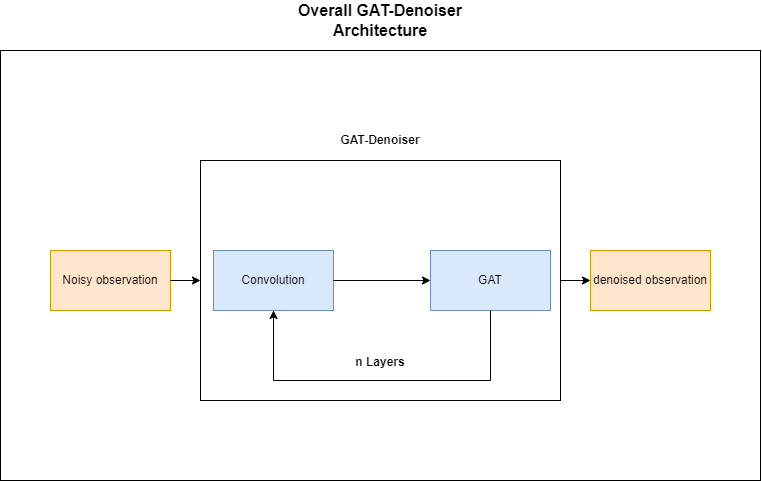
\includegraphics[width=0.6\textwidth]{Overall_final_Architecture.drawio.png}
  \caption{Overall GAT-Denoiser architecture}
\end{figure}

In figure~\ref{fig:architecture-overall}, the overall GAT-Denoiser architecture is illustrated.
GAT-Denoiser is a GNN and has two main components, namely convolution layers and GAT layers.
For a given noisy observation $y$, $y$ will process the network and result in a denoised version.

GAT will be responsible to average over observation neighbours, but single observations will
not be averaged by the GAT. 
Therefore, convolution is added and is responsible to denoise single observations
before averaging over neighbourhood with GAT. So for every GAT layer, there is a preceding convolution. 
In the case of computed tomography, this will be a 1D convolution, in case of cryo-EM a 2D convolution.

\paragraph{K-hop neighbourhood:}
In GNNs, multiple layers expose the k-hop neighbourhood. So a network with $k$ layers,
the network operates on the $k$-hop neighbourhood.


\subsection{Layers}

In figure~\ref{fig:architecture-detailed}, the detailed GNN architecture can be seen.
It is paremetrized with $channels$, $heads$ and $layers$. 
The number of channels in convolution can be increased with parameter $channels$.
Fruther, $heads$ determine the number of heads used in the GAT layers and parameter 
$layers$ defines how many convolution and GAT layers are stacked together.


\begin{figure}[H]
  \centering
  \label{fig:architecture-detailed}
  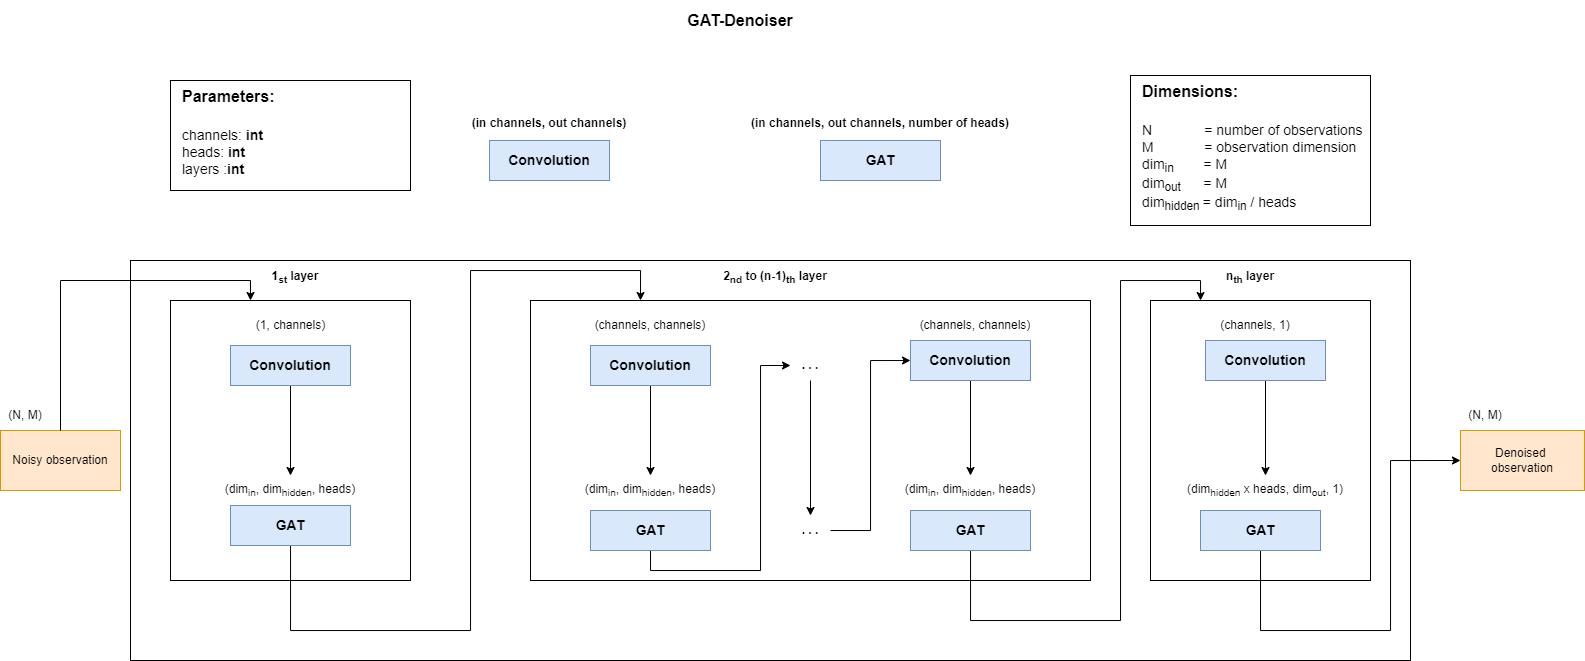
\includegraphics[width=\textwidth]{GAT_Architecture_Detail.drawio.png}
  \caption{Overall GAT-Denoiser architecture}
\end{figure}


For every layer, first convolution and then GAT is processed. 
Convolution in the whole network was defined with kernel size of 3 and padding 1,
therefore, the dimension of convolved signal will not change.
Further, additional convolutional channels can be used for learning.
If parameter $channels$ is set $ > 1$, channels are increased in the first convolution layer 
and decreased in the last one.
Parameter $heads$ controls the multi-head approach for GAT. Input and hidden dimension
of GAT is set to size of sampling points (sinogram resolution) if no heads are used.
If multi-head attention is used, hidden dimension will be set to $dim_{in} / heads $.
In the last GAT layer, everything gets prepared for output dimension and 
averaging with only 1 head is applied.




\subsection{Training}

As already mentioned, an end-to-end learning approach is used where quality of reconstruction is 
compared in the loss.

Therefore, the outcom of GAT-Denoiser is not directly part of the loss, but first reconstruction will be computed.
Reconstructions can be nicely compared with the $\ell2$-norm:

\begin{equation}
  \mathcal{L} = || x_i - Recon ( \text{GAT-Denoiser}(A(x_i, \theta, s) + \eta)) ||^2_2
\end{equation}

As $x_i$ is part of the loss, access to original object is needed during training.

Further, U-Net will be jointly used with FBP as reconstruction. For that to work, U-Net needs to be 
first trained with the dataset and learned model can be be pluged into GAT-Denoiser.

The overall learning pipeline is illustrated in figure~\ref{fig:pipeline-overall}.

\begin{figure}[H]
  \centering
  \label{fig:pipeline-overall}
  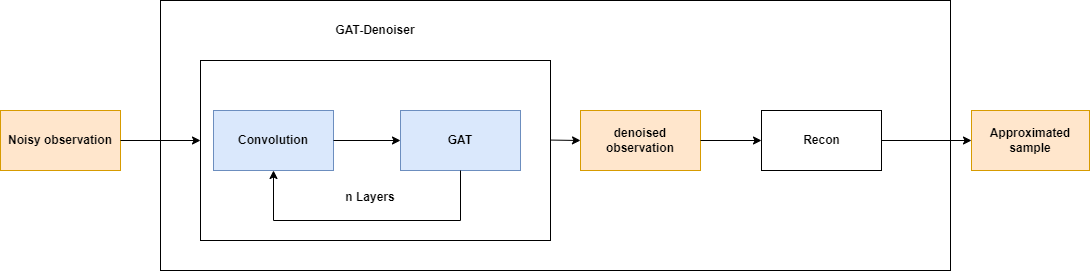
\includegraphics[width=\textwidth]{Overall_GAT-Denoiser_Pipeline.drawio.png}
  \caption{Overall GAT-Denoiser learning pipeline}
\end{figure}







